\documentclass[cn,11pt,chinese,toc=twocol]{elegantbook}
\title{利息理论}
\subtitle{made by \LaTeX{} }
\author{Icecream}
\cover{cover14.pdf}
% 本文档命令
\usepackage{tikz}
\usepackage{mathpazo} 
\usepackage{array}
\newcommand{\ccr}[1]{\makecell{{\color{#1}\rule{1cm}{1cm}}}}

\begin{document}
\def\angles#1{{%
		\vbox{\hrule height .2pt
			\kern 1pt
			\hbox{$\scriptstyle {#1}\kern 1pt$}%
		}\kern-.05pt \vrule width .2pt
}}
%
\maketitle
\tableofcontents

\chapter*{Introduction}
\markboth{Introduction}{Introduction}
\noindent 保险精算研究的对象是年金,现金流和债券,年金的性质是研究现金流和债券的基础.\\
利息理论是精算专业的一门基础课. 几乎所有国家和地区的精算师资格考试都会涉及该门课程的内容。最近几年. 国际上主要的精算师协会[如北美寿险精算师协会(SOA)、北美非寿险精算师协会(CAS) 和中国精算师协会]在精算师资格考试中都把该门课程更名为金融数学. 但利息理论仍然是其主体. 只是在此基础上增加了金融衍生产品的一些基本内容。
\\在金融学和财务管理等专业课程中. 都会涉及利息理论的一些基本内容. 但对这部分内容的介绍各有侧重, 系统性不够. 不易形成完整的利息理论知识体系。利息理论课程把这类蜇化分析方法整合在一起, 可以在一定程度上提高教学效率, 同时可以
避免不同课程在这部分内容上的重复。
\chapter{利息度量}
\begin{introduction}
	\item 累积函数
	\item 贴现
	\item 利息力
\end{introduction}
		\section{累积函数}
	\begin{definition}{累积函数}
\noindent 	时间零点的1元在时间t的累值,记为 $a(t)$
		\end{definition}
\begin{property}
  \noindent  (1) $a(0)=1$\\
(2) $a(t)$ 通常是时间的增函数\\
(3) 当利息连续产生时, $a(t)$ 是时间的连续函数
\end{property}
	\section{贴现}
	\begin{definition}{贴现}
\noindent	$v=\frac{1}{1+i}$ \\ $d=iv$\\ $i=\frac{1}{v}-1$
	\end{definition}
\begin{note}
i:利率,v:贴现因子,d:贴现函数
\end{note}
\begin{definition}{利息力}
\noindent		设可积函数连续可导,则称
\[
\delta_{t}=\frac{a^{\prime}(t)}{a(t)}=[\ln a(t)]^{\prime}
\]
为时刻 t 的利息力
		\end{definition}
		\\ 衡量利息增长速率与利息本身大小的比值
		很有意思的是,我们把t当做横坐标的时候,相当于t是定下来的,以这个为标准来用利息力来计算累积函数
		$$\int_{0}^{t} \delta_{s} d s=\int_{0}^{t} \frac{a^{\prime}(s)}{a(s)} d s=\int_{0}^{t}[\ln a(s)]^{\prime} d s=\ln a(t)$$
		\begin{property}
		$$\ln \left(a\left(t_{2}\right)\right)-\ln \left(a\left(t_{1}\right)\right)=\int_{t_{1}}^{t_{2}} \delta_{t} d t \text { or } a\left(t_{2}\right)=a\left(t_{1}\right) e^{\int_{t_{1}}^{t_{2}}\left(\delta_{t}\right) d t}$$
\\We can also write, assuming that $a(0)=1$
\[
\ln (a(t))=\int_{0}^{t} \delta_{\tau} d \tau \text { or } a(t)=e^{\int_{0}^{t} \delta_{\tau} d \tau}
\]
\end{property}
\begin{property}
	累积函数:\\
\[
a(t)=\exp \left(\int_{0}^{t} \delta_{s} d s\right)
\]\\
 贴现函数:\\
\[
a^{-1}(t)=\exp \left(-\int_{0}^{t} \delta_{s} d s\right)
\]
	\end{property}
Timeline:a essentail point of view for problem-solving \\
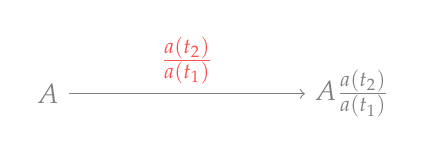
\begin{tikzpicture}
\draw [color=black!50,->](0,0) node[left]{$A$}-- node [color=red!70,pos=0.5,above,sloped]{$\frac{a(t_2)}{a(t_1)}$}(3,0) node[right]{$A\frac{a(t_2)}{a(t_1)}$};
 \end{tikzpicture}
\begin{example}
compound interest:$a(t)=(1+i)^t$\\
$$A \cdot \frac{a\left(t_{2}\right)}{a\left(t_{1}\right)}=A(1+i)^{t_{2}-t_{1}}$$
\end{example}
\begin{example}
simple interest:$a(t)=1+it$\\
$$A \cdot \frac{a\left(t_{2}\right)}{a\left(t_{1}\right)}=A \cdot \frac{1+i t_{2}}{1+i t_{1}}$$
\end{example}
\
$$(1+\frac{i^{(n)}}{n})^{n}=(1+\frac{i^{(m)}}{m})^{m}$$
\begin{exercise}
	在第1月末支付314元的现值与第18月末支付271元的现值之和,等于在第T月末支付1004元的现值.年实际利率为$5\%$. 求$T$
\end{exercise}
\begin{solution}
$$1004 v^{T / 12}=314 v^{1 / 12}+271 v^{18 / 12} \Rightarrow T=141.6$$
\end{solution}
\chapter{等额年金}
\begin{introduction}
	\item 每年支付m次的年金
	\item 连续支付的等额年金
\end{introduction}
\section{符号一览}
\noindent$a_{\angles{n}},s_{\angles{n}}$\\	$\ddot{a}_{\angles{n}}$\\$\ddot{s}_{\angles{n}}$
\section{等额年金}
\begin{definition}{年金的终值与现值}
\noindent $a_{\angles{n}},s_{\angles{n}}$\\
$s_{\angles{n}}=a_{\angles{n}}(1+i)^{n}=\frac{(1+i)^{n}-1}{i}$
\end{definition}
\begin{definition}{Accumulated Value of an $n$ -Payment Annuity-Immediate of 1 Per Period}

	The symbol $s_{\angles{n}}$ denotes the accumulated value, at the time of (and including) the final payment of a series of $n$ payments of 1 each made at equally spaced intervals of time, where the rate of interest per payment period is $i$
	$\begin{aligned}
	s_{\angles{n}} &=(1+i)^{n-1}+(1+i)^{n-2}+\cdots+(1+i)+1 \\
	&=\sum_{t=0}^{n-1}(1+i)^{t}=\frac{(1+i)^{n}-1}{i}
	\end{aligned}$
\end{definition}
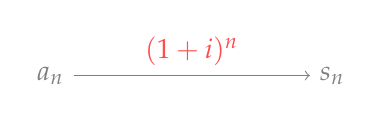
\begin{tikzpicture}
\draw [color=black!50,->](0,0) node[left]{$a_{\angles{n}}$}-- node [color=red!70,pos=0.5,above,sloped]{$(1+i)^n$}(3,0) node[right]{$s_{\angles{n}}$};
    \end{tikzpicture} \\
\noindent $a_{\angles{n}}=v+v^2+v^3+\dots+v^n=\frac{1-v^n}{i}=\frac{1-\frac{1}{(1+i)^n}}{i}=\frac{1-v^n}{\frac{1}{v}-1}$\\
\begin{lstlisting}[language={python}]
#wolframalpha
(1-(1/(1+i)^n))/i=(1-v^n)/(1/v-1)
\end{lstlisting}
$\ddot{a}_{\angles{n}}=\frac{1-v^n}{d}$ \\
$s_{\angles{n}}=a_{\angles{n}}(1+i)^{n}=\frac{(1+i)^{n}-1}{i}$\\
$\ddot{s}_{\angles{n}}=\ddot{a}_{\angles{n}}(1+i)^{n}=\frac{(1+i)^{n}-1}{d}$
\begin{property}
$1=i{a}_{\angles{n}}+v^n$
\end{property}
\begin{property}
$$\begin{array}{l}
\ddot{a}_{\angles{n}}=a_{\angles{n}} \times(1+i) \\
\ddot{a}_{\angles{n} }=a_{\angles{n-1} |+1 \\
\ddot{S}_{\angles{n} }=S_{\bar{n}} \times(1+i) \\
\ddot{S}_{\angles{n}}=S_{\angles{n+1} }-1
\end{array}$$
\end{property}
 \begin{definition}{每年支付m次年金}
\noindent ${a}_{\angles{n}}^{(m)}=\frac{1-v^n}{i^{(m)}}$ 
 \end{definition}
 \section{永续年金(Perpetuity)}
 期初付永续年金的现值
\[
\ddot{a}_{\angles{\infty}}=1+v+v^{2}+\cdots=\frac{1}{1-v}=\frac{1}{1-v}=\frac{1}{d}
\]
期末付永续年金的现值
\[
a_{\angles{\infty}}=v+v^{2}+\cdots=\frac{1}{1-v}=\frac{v}{1-v}=\frac{v}{d}=\frac{v}{i v}=\frac{1}{i}
\]
与有限年金的联系
\[
\begin{array}{c}
\ddot{a}_{\angles{\infty}}=\lim _{n \rightarrow \infty} \ddot{a}_{\pi}=\lim _{n \rightarrow \infty} \frac{1-v^{n}}{d}=\frac{1}{d} \\
a_{\angles{n}}=\frac{1-v^{n}}{i}=\frac{1}{i}-v^{n} \frac{1}{i}=a_{\angles{\infty}}-v^{n} a_{\angles{\infty}} \Leftrightarrow a_{\infty}=a_{\angles{\infty}}+v^{n} a_{\angles{\infty}}
\end{array}
\]
对期初付年金也有相应的关系: $\ddot{a}_{\angles{\infty}}=\ddot{a}_{\pi}+v^{n} \ddot{a}_{\angles{\infty}}$

\chapter{紧致性}
\begin{definition}{cover}
A collection $\mathcal{A}$ of subsets of a space $X$ is said to cover $X,$ or to be a covering of $X,$ if the union of the elements of $\mathcal{A}$ is equal to $X .$ It is called an open covering of $X$ if its elements are open subsets of $X$
\end{definition}
\begin{definition}{compact}
A space $X$ is said to be compact if every open covering $\mathcal{A}$ of $X$ contains a finite subcollection that also covers $X$
\end{definition}
\begin{theorem}
Every closed subspace of a compact space is compact.
\end{theorem}
\chapter{收益率}
\begin{introduction}
	\item 收益率
	\item 基金的利息度量
	\item 再投资
	\item 基金
\end{introduction}
\section{收益率}
已知一个项目的现金流,如何评价其收益水平的高低?\\
\subsection{净现值}
(1) 净现值法 (net present value, NPV)
\[
N P V(i)=\sum_{t=0}^{n} v^{t} R_{t}=\text { 资金流入现值 }-\text { 资金流出现值 }
\]
\subsection{收益率法}
资金流入的现值与资金流出的现值之差就是净现值,所以收益率也是使得净现值等手零的利率:
\[
N P V(i)=\sum_{t=0}^{n} v^{t} R_{t}=0
\]
\section{基金的利息度量}
\begin{definition}{币值加权收益率}
\noindent	Suppose the following information is known:
	(i) the balance in a fund at the start of the year is $A$ \\
	(ii) for $0<t_{1}<t_{2}<\cdots<t_{n}<1,$ the net deposit at time $t_{k}$ is amount $C_{k}$ (positive for a net deposit, negative for a net withdrawal), and \\
	(iii) the balance in the fund at the end of the year is $B$
	Then the net amount of interest earned by the fund during the year is $I=B-\left[A+\sum_{k=1}^{n} C_{k}\right],$ and the dollar-weighted rate of return earned by the fund for the year is
	\[
	\frac{I}{A+\sum_{k=1}^{n} C_{k}\left(1-t_{k}\right)}
	\]
	\\---度量投资者的业绩
\end{definition}
\begin{remark}
	$(Ia)_{\angles{n}}=\frac{\ddot{a}_{\bar{n}}-n v^{n}}{i}$
\end{remark}
\begin{definition}{时间加权收益率}
\noinent Suppose the following information is known:\\
	(i) the balance in a fund at the start of the year is $A$\\
	(ii) for $0<t_{1}<t_{2}<\cdots<t_{n}<1,$ the net deposit at time $t_{k}$ is amount $C_{k}($ positive for a net deposit, negative for a net withdrawal)\\
	(iii) the value of the fund just before the net deposit at time $t_{k}$ is $F_{k},$ and\\
	(iv) the balance in the fund at the end of the year is $B$
	The time-weighted return rate earned by the fund for the year is
	\[
	\left[\frac{F_{1}}{A} \times \frac{F_{2}}{F_{1}+C_{1}} \times \frac{F_{3}}{F_{2}+C_{2}} \times \cdots \times \frac{F_{k}}{F_{k-1}+C_{k-1}} \times \frac{B}{F_{k}+C_{k}}\right]-1
	\]	
	\\度量基金经理人的业绩
\end{definition}	
\section{再投资}
\begin{example}
期初投资 1 元,投资期限为 $n$ 年, 年实际利率为 $i$ ,如果每年产生的利息按照年实际利率 $j$ 进行用投资, 试计算在第 $n$ 年末的累积值与该项投资的年平均收益率。
\end{example}
\begin{solution}
(1) 该投资在第 $n$ 年末的黑积值为 $1+i \cdot s_{\angles{n} j}$\\
(2) 假设该项投资的年平均收益率为 X,则由价值方程
\[
1+i \cdot s_{\angles{n} j}=(1+x)^{n} \Longrightarrow x=\left(1+i \cdot s_{\angles{n} j}\right)^{\frac{1}{n}}-1
\]
特别地,当 $j=i$ 时 $, x=i$
\end{solution}
\subsection{修正收益率}
如果再投资的利率与筹集资金的利率不同时,则评价项且应该使用修正收益率 (modified rate of internal rate) 在计算修正收益率时\\
对资金流出使用筹资的利率计算其现值\\
对资金流入使用再投资的利率计算其累积值
\section{基金}
\noindent 基金的收益:
\\收入:利息(债券,银行存款)、股息、资本利得(股票价格上涉)
\\净收益: 收入 - 费用
基金包括不同时期投资,如何把基金收入分配给不同时期的投资?
\\分配方法:
\\投资组合法 (portfolio method)
\\投资年度法 (investment year method)
\chapter{债务偿还方法}
\begin{introduction}
	\item 等额分期偿还
	\item 等额偿债基金
	\item 变额分期偿还
\end{introduction}
\section{分期偿还法}
\subsection{等额分期偿还}
\noinent 每次偿还的金额:$R=\frac{L_0}{a_{\angles{n}}}$\\
未偿还本金:$L_k=Ra_{\angles{n-k}}=L_0(1+i)^k-Rs_{\angles{k}}$\\
\\ 支付的本金:
支付的利息:$I_k=iL_{k-1}=iRa_{\angles{n-k+1}}=R(1-v^{n-k+1})$\\
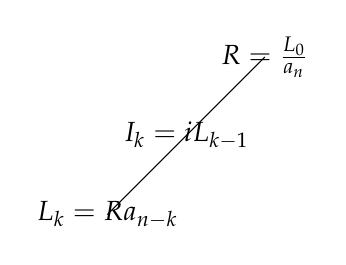
\begin{tikzpicture}
\draw (1,1) node{$L_k=Ra_{\angles{n-k}}$} -- (2,2) node{$I_k=iL_{k-1}$}-- (3,3) node{$R=\frac{L_0}{a_{\angles{n}}}$};
\end{tikzpicture}
\begin{exercise}
贷款一笔钱,n年内等额分期付款,每年末还一次,偿还金额是X,第一年利息是604RMB,第三年是593.75,第五年利息是582.45,计算X
\end{exercise}
\begin{note}
支付的利息:$I_k=iL_{k-1}=iRa_{\angles{n-k+1}}=R(1-v^{n-k+1})$
\end{note}
\begin{exercise}
按年实际利率i偿还一笔 1000 元的贷款。已知:\\
(1)在第6年末偿还第一笔款项\\
(2)然后每年未等额偿还一次在第15年末可以偿清这笔贷款(即一共偿还 10 次)\\
(3)在第10年末的付款结束后。未偿还本金余额为 908.91 元\\
试计算第5年末的未偿还本金余额
\end{exercise}
\begin{solution}
设等额付款金额为 $R: Ra_{\angles{5}i}=908.81, Ra_{\angles{10}}=1000(1+i)^5 \\
故第5年末的未归还本金为 $1000 \times(1+i)^{5}=1510.6$ 元
\end{solution}
\section{等额偿债基金}
区别:偿还本金采用不同的计息方式\\
$$D=\frac{L_0}{s_{\angles{n}j}}$$\\
$$R=I+D$$\\
$$L_k=L_0-Ds_{\angles{n}j}$$
\chapter{债务价值分析}
\begin{introduction}
	\item 定价公式
	\item 等额偿债基金
	\item 变额分期偿还
\end{introduction}
\section{符号一览}
\noindent $P:$ 债券价格 (bond price) \\
$i$ :债券的到期收益率(yield-to-maturity rate),即投资人购买债券者购买债券所要求的收益率\\
$F :$ 债券的面值 (par value,face amount, nominal value),即债券到时支付给债券持有人的金额,也称为票面价值或到期值\\
$r:$ 债券的息票率 (coupon rate per payment period)\\
$rF$ 息票收入 \\
$i_{c}:$ 债券的当期收益率: $i_{c}=\frac{r F}{P}$\\
$C :$ 债券的偿还值 (redemption payment),通常等于侦券面值F\\
$n$ : 息票的支付次数 (number of coupon payments)\\
$g:$ 债券的修正息票率, $g=\frac{r F}{C}$\\
债券定价原理:到期偿还值+债券未来息票
$$P=rFa_{\angles{n}}+Cv^n$$
\begin{note}
\begin{aligned}
\frac{\partial P}{\partial i} &=-\left(\sum_{t=1}^{n} r F t v^{t+1}+C n v^{n+1}\right)<0 \\
\frac{\partial^{2} P}{\partial i^{2}} &=\sum_{t=1}^{n} r F t(t+1) v^{t+2}+C n(n+1) v^{n+2}>0
\end{aligned}
\end{note}
\noindent 定价公式主要包含:\\
(1) 基本公式 \\
(2) 溢价公式 \\
(3) 基价公式 \\
(4) Makeham 公式
$$P=\left\{\begin{array}{ll}
r F a_{\angles{n}}+C v^{n} & \text { 基本公式 } \\
C+C(g-i) a_{\angles{n}} & \text { 溢价公式 } \\
G+(C-G) v^{n} & \text { 基价公式 } \\
\frac{g}{i}(C-K)+K & \text { Makeham 公式 }
\end{array}\right.$$
(1) 息票率:
$$r=\frac{\text { 息票收入 }}{\text { 面值 }(F)}$$
(2) 修正息票率:
$$g=\frac{\text { 息票收入 }}{\text { 偿还值 }(C)}$$
(3) 到期收益率:
$$i=\frac{\text { 息票收入 }}{\text { 基价 }(G)}$$
(4) 当期收益率:
$$i_{c}=\frac{\text { 息票收入 }}{\text { 债券价格 }(P)}$$
\chapter{利率风险}
\begin{definition}{利息力}
\noindent		设可积函数连续可导,则称
\[
\delta_{t}=\frac{a^{\prime}(t)}{a(t)}=[\ln a(t)]^{\prime}
\]
为时刻 t 的利息力
		\end{definition}
		\\ 衡量利息增长速率与利息本身大小的比值
		很有意思的是,我们把t当做横坐标的时候,相当于t是定下来的,以这个为标准来用利息力来计算累积函数
		$$\int_{0}^{t} \delta_{s} d s=\int_{0}^{t} \frac{a^{\prime}(s)}{a(s)} d s=\int_{0}^{t}[\ln a(s)]^{\prime} d s=\ln a(t)$$
\section{Macaulay duration}
	\begin{definition}{Macaulay duration}
$$D_{\text {麦 }}=\frac{\sum_{t>0} t \cdot R_{t} e^{-\delta t}}{\sum_{t>0}  \cdot R_{t} e^{-\delta t}}$$
\end{definition}
\begin{note}
一笔 $n$ 年期贷款,年实际利率为 $i,$ 按年等额分期偿还,求该笔贷款的麦考利久期。
\end{note}
\begin{solution}
$$\begin{aligned}
D_{\text {麦 }} &=\frac{\sum\limits_{t>0} t \cdot R(1+i)^{-t}}{\sum\limits_{t>0} R(1+i)^{-t}}=\frac{(I a)_{\angles{n }}}{a_{\angles{n }}}} \\
&=\frac{\ddot{a}_{\angles{n}}-n v^{n}}{i \cdot a_{\angles{n }}}=\frac{(1+i) a_{\angles{n }}}{i \cdot a_{\angles{n }}}-\frac{n v^{n}}{i \cdot \frac{1-v^{n}}{i}} \\
&=\frac{1+i}{i}-\frac{n}{(1+i)^{n}-1}
\end{aligned}$$
\end{solution}
\subsection{修正久期}
\begin{definition}{修正久期}
$$D=\frac{D_{\text {麦 }}}{1+\frac{y}{m}}$$
\end{definition}
\begin{note}
	债券面值为F,期限为n,到期时按面值偿还,年息票率为r,到期收益率r,求$D_{\text {麦 }$\\
		$$D_{\text {麦 }}=\frac{\sum_{t=1}^{n}tv^trF+nv^nF}{\sum_{t=1}^{n}rFv^t+v^nF}$$
		$$=\frac{\sum_{t=1}^{n}tv^tr+nv^n}{\sum_{t=1}^{n}rv^t+v^n}$$
\end{note}
\begin{exercise}
某 2 年期债券的面值为 1000 元,年息票率为 8%,每半年末支付一次利息,债券到期按面值偿还。该债券每半年复利一次的到期收益率为4%,请计算该债券的修正久期
\end{exercice}
\begin{solution}
该债券的价格为
$$P=2 \times 40 a_{\angles{2}4 \%}^{(2)}+1000 \times(1+4 \% / 2)^{-4}=1076.16(\text { 元 })
$$
麦考利久期为
$$D_{\text {麦 }}=\frac{\sum_{t>0} t \cdot R_{t}(1+i)^{-t}}{P}=\frac{2036.19}{1076.16}=1.89$$
修正久期:$$D=\frac{D_{\text {麦 }}}{1+i^{(2)} / 2}=\frac{1.89}{1+4 \% / 2}=1.86$$
\end{solution}
\end{document}
